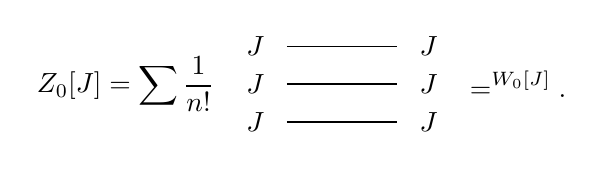
\begin{tikzpicture}[x=1cm,y=1cm,baseline=(current bounding box.center)]
  \node[anchor=east] at (0.15,0) {$\displaystyle Z_0[J]=\sum\frac{1}{n!}$};
  % three disconnected free propagators, each running between two sources J
  \foreach \y in {0.48,0,-0.48} {
    \node at (0.55,\y) {$J$};
    \draw[line width=.55pt] (0.95,\y) -- (2.35,\y);
    \node at (2.75,\y) {$J$};
  }
  \node[anchor=west] at (3.15,0) {$\displaystyle =\ee^{\ii W_0[J]}.$};
\end{tikzpicture}
